%
% PKUMpLtX --- A LaTeX document class for 'Modern Physics Laboratory' in PKU based on `revtex4-2`
%
% Please read `README.md' and the template file before using
\documentclass[font=notofandol]{mpltx}

% 以下三行仅为本文件额外定义的命令
\hypersetup{colorlinks=true}% 超链接带颜色
\usepackage{xcolor}
\newcommand{\note}[1]{{\color{gray}#1}}

\begin{document}

\title{实验题目} % 切合报告内容, 简短明确, 可以不同于讲义
\author{姓名} % 这里 \emailphone 一定要紧跟在 \author 后方
\emailphone{email@pku.edu.cn}{(86)152XXXXXXXX}
% 如果改用 \email 则仅需要邮箱参数
\affiliation{北京大学物理学院\quad 学号: 20000xxxxx}
% % 可以使用 \zhdate 自动生成中文日期, 如
% \date{\zhdate{2020/12/1}}
% % 也可使用 babel 的 \localedate, 如
% \date{\localedate{2020}{12}{1}}
% % 两者均会输出 `2020 年 12 月 1 日'
% 下面这行是为了自动输出正确版本号, 正式报告请替换为上面的两种 \date 之一
\makeatletter\date{\mpltx@filedate, \mpltx@fileversion}\makeatother

\begin{abstract}
    此部分为摘要.
    200--300字, 说明用什么方法做了什么事, 由此得到什么结果和结论, 有何意义.
    摘要中不用缩略词, 不用第一人称.
    \note{本文档为对 \textsf{PKUMpLtX} 的使用示例, 灰色部分为额外针对 \LaTeX{} 模板使用的说明.
        也请注意查看源文档 \texttt{template.tex} 中的注释.}
\end{abstract}
\keywords{关键词1, 关键词2, 共2--4个}

\maketitle

\section{引言}

研究论文引言一般包含以下内容:
所研究领域背景和现状,
有待研究的问题,
本研究的物理目的和主要方法.
% 通过空行或者 \par 命令分段
引言一定要切合报告正文, 不能漫无目的地介绍背景, 要快速地将读者引导到报告主题上.
引言篇幅可以在较大范围内变化, 但最长不应超过报告文字篇幅的1/3.

引言撰写可以参考实验讲义和资料, 可以概括复述, 但不能抄.
\note{这里是一个对实验教材 \cite{jindaishiyan} 的引用示例.}
\note{注意在 \texttt{\textbackslash{}cite\{\}} 命令前后适当添加空格.
    可以连续引用.
    引用标记要出现在在句子结束的标点之前 \cite{jindaishiyan,zamojski2007deep}.}

\section{理论}\label{sec:theory}

可选, 概括本实验必须的理论.
也可以适当地给出必要的公式, 公式应编号.
\note{自然对数的底和虚数单位国标和 ISO 都推荐为正体 (虽然国际学界并不怎么实行这点), 本模板提供了 \texttt{\textbackslash{}ii}, \texttt{\textbackslash{}ee}, \texttt{\textbackslash{}jj} 作为简写, 如
    \begin{equation}\label{eq:1}
        \ee^{\ii\pi}+1=0.
    \end{equation}
    注意公式应作为句子的一部分在末尾给出必要的标点符号.
    上式可以交叉引用为\autoref{eq:1}.}

\note{此外, 摄氏度和度在2020年初后已可在 \LaTeX{} 中的非数学模式直接打出, 比如 \texttt{\textbackslash{}textdegree} (\textdegree) 和 \texttt{\textbackslash{}textcelsius} (\textcelsius, 虽然 Unicode 更推荐使用\texttt{\textbackslash{}textdegree\{\}C}的写法, 写成\textdegree{}C).
    再比如, \texttt{\textbackslash{}textmu} (\textmu) 可以给出微米需要的正体词头符号.
    你也可以使用 \textsf{siunitx} 宏包 (参见 \texttt{README.md}) 来帮助你管理单位格式.}

\section{实验装置}
在此部分需要成段介绍实验方法和条件 (不是罗列操作步骤), 交待清楚到别人能重复你的实验结果的程度.
此外, 还需表明你已尽了最大努力来提高实验精度和结果的可靠性 (简单的不确定度估计可以在此节给出, 复杂一些的可以放到分析讨论部分).

首先应给出一个实验装置示意图.
例如, 如下同学的示意图\autoref{fig:instruments} 非常清晰, 值得借鉴 (各关键部件也可标在图中).

\begin{figure}
    \centering
    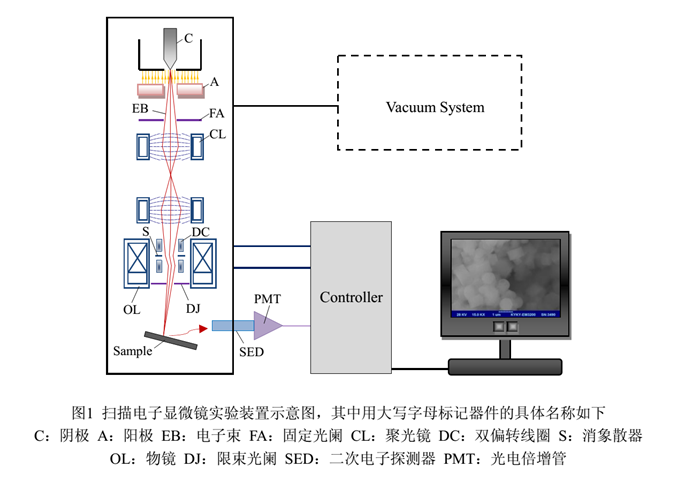
\includegraphics[width=0.85\linewidth]{fig/instruments.png}
    \caption{这个例子展示了如何插入图片以及加标题和标签.
        \note{推荐使用相对大小插入图片, 比如这里是 0.8 倍当前区域文字宽度 (\texttt{\textbackslash{}linewidth}).
            推荐对实验装置图和数据图使用矢量图插入}}
    \label{fig:instruments}
\end{figure}

\note{这里使用了 \texttt{\textbackslash{}autoref\{\}} 命令来自动给出带类型的交叉引用, 注意在命令前后适当使用空格以给出最好的显示效果.
    小节, 表格, 公式等都可如此引用, 如: \autoref{sec:theory}, \autoref{ssec:table}, \autoref{sssec:table}, \autoref{eq:1}, \autoref{tab:table_eg}, \autoref{app:exercise}, \autopageref{tab:table_eg}.
    交叉引用的标签尽量取得有意义.}

实验仪器和方法不是像普物实验报告那样将所有实验器材列出, 而是要用介绍功用的方式成段给出.
实验条件不仅是指直接影响实验结果的实验参量, 而且还包括影响实验质量和可靠性的因素, 如室温、空气湿度、基真空、原材料纯度等.

\section{结果及讨论}

此部分是实验报告的主体, 应占报告篇幅的一半以上.
\note{依自己意愿, 结果与分析部分可以分多个小节, 甚至可以将实验结果和对结果的分析讨论拆分为两节.}

实验结果应尽量以图表的形式给出. 每一个图表都应该是完整的, 即阅读图表时可以不必依赖正文.
以图表为中心叙述实验结果和讨论.

\subsection{表格}\label{ssec:table}
\subsubsection{表格}\label{sssec:table}


表是被一系列横线隔开的有序排列的数据, 报告格式要求最上和最下两条横线为双横线.
\note{此双横线格式可以通过 \texttt{ruledtabular} 环境和 \texttt{\textbackslash{}colrule} 命令实现.}
例表为\autoref{tab:table_eg}.

\begin{table}
    \caption{表格示例
        \footnote{表格标题要简明扼要; 注意使用 \textsf{revtex} 提供的 \texttt{ruledtabular} 环境生成首尾双横线的表格.
            表格中的脚注会自动加在表尾.
            为方便, 提供了 \texttt{\textbackslash{}mc} 作为 \texttt{\textbackslash{}multicolumn} 的简写.
            \href{https://www.tablesgenerator.com}{Tables Generator 网站}可以方便地生成 \LaTeX 表格.}}
    \label{tab:table_eg}
    \begin{ruledtabular}% ruledtabular 环境自动生成首尾双横线, 并调整宽度至占满全行
        \begin{tabular}{cd{4.2}lr}
            % d{a.b} 能使该列中的数据按小数点对齐, 前方留 a 个字符, 后方留 b 个字符
            % 已将 multicolumn 简写为 mc
            居中    & \mc{1}{c}{数值\footnote{``数值'' 列使用了 \texttt{d} 列格式来按小数点位置对齐. 记得将 d 列的列标题单独设为居中.}} & 靠左    & 靠右 \\
            \colrule% 中间横线
            a     & 0.12                                                                            & a     & a \\
            bbb   & -100                                                                            & bbb   & bbb \\
            ccccc & 50.8                                                                            & ccccc & ccccc
        \end{tabular}
    \end{ruledtabular}
\end{table}

从\autoref{tab:table_eg} 可以看出, 对表中各项的注释应作为表的一部分放在表后, 而不是页脚或文尾.
\note{在表格中使用 \texttt{\textbackslash{}footnote\{\}} 命令时 \LaTeX 会自动将注释放在表尾.
    但正文中的注释按照 AIP 的要求 (以及 \textsf{revtex} 的实现) 是会和各引用项共同编号并作为参考文献列表的一部分的.
    因此, 只要你在正文使用了 \texttt{\textbackslash{}footnote\{\}}, 即使你没有引用任何文献 (这一般不太可能), 也需要用 B\textsc{ib}\TeX 处理.
    这里是一个尾注的例子 \footnote{这里是一个尾注的例子}.}

当原始数据和处理过的数据常需要出现在同一表中时, 用软件来处理会非常方便.
但出现在实验报告中的表应具有上面给出的例子的格式.

\subsection{数据图}

\textbf{每个图应尽量让读者不看正文就能基本理解图的含意.}
应包含: 图名、轴名、轴、刻度、标尺、数据点、曲线、图例、标注和图注等部分.
最常用的作图软件有 Origin 或 MATLAB.
学习使用基本的数据处理和作图工具软件也是课程的基本内容.
课程也鼓励大家使用 Python 语言编程作图.
逐点测量得到的函数关系要同时用表格和图给出.
\note{数据点过多可以将数据放到附录.
    这里 ``逐点测量得到的函数关系'' 还是要自己把握一下, 像那种几千个数据点的能谱当然就没必要放原始数据表了.}
\textbf{需要作比较的多条曲线要画在同一图上.}
为避免读者在图表和正文间反复跳跃阅读, 正文叙述应紧邻图表, 正文中也要对图表作必要的说明.

\begin{figure}
    \centering
    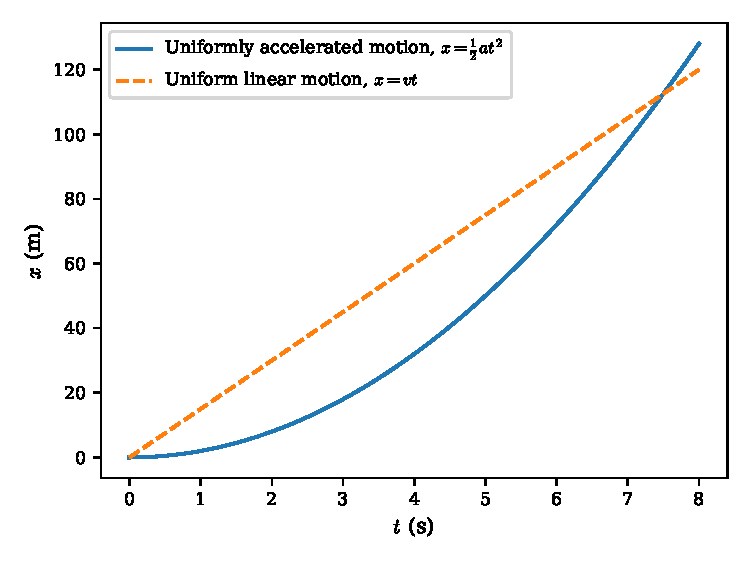
\includegraphics[width=0.8\textwidth]{fig/figsample.pdf}
    \caption{这是数据图的例子.
        \note{在图的 \texttt{\textbackslash{}caption\{\}} 中应简要说明图中表达的内容, 并对各种符号、线型、颜色的意义做出说明.
            如果有多格数据图, 应清晰地分别做出解释说明.
            图中的关键性文字 (比如轴名和图例) 的大小最好能和 caption 中的文字大小相当.
            关于坐标轴名和单位的标法, 可以参看\href{https://journals.aps.org/authors/axis-labels-and-scales-on-graphs-h18}{美国物理学会的说明}.
            本图是用脚本 \texttt{./figgen.py} 生成的}}
    \label{fig:data}
\end{figure}

\autoref{fig:data} 是一张例图.

\subsection{对分析的要求}

对于预料之外的实验结果, 必须首先小心证明其可靠性.
读者只有在相信你的实验结果时才愿意花时间看你的分析.

\textbf{必须用文字归纳整理出正式的实验结果或结论.}
可信的实验结果是课程报告最重要的内容.
作为一个实验物理工作者, 分析解释出错并不丢脸, 实验结果不被采信则是致命的.
教学实验的结论往往是预先知道的.
所以, 教师更关心的是你的说理过程.
一般说来, 单由课内实验的结果不足以能得到明确的结论.
此时, 你可以引用他人的研究结果来帮助帮助自己的论证, 但必须注明出处.
确实不能得到明确结论时, 可以给出几种可能结论并指出可以再做哪些实验来帮助作进一步的判断.
总之, 分析讨论部分要做到: 论据要valid, 论证要reasonable, 结论要convincing.

\section{结论}
\textbf{文字写一段.}
首先要给出实验结果, 然后再给出由实验结果分析得到的结果和结论.
此部分给出的内容要比摘要中的全面, 用词要更准确.

\begin{acknowledgments}
    感谢对实验和报告有具体重要帮助的, 又没被列为作者的人.
    \note{撰写致谢时请使用 \texttt{acknowledgments} 环境.}
\end{acknowledgments}

% bibliography 的参数是你的 *.bib 文件去掉后缀名后的部分
\bibliography{bibli}

\clearpage % 附录前另起一页
\appendix % 附录开始
\section{思考题}\label{app:exercise}
\subsection{可以把每道思考题的题目分别作为小标题}
然后书写解答.

\section{近代物理实验报告写作要求}

物理实验的结果最终需要以论文或报告的形式向同行或公众报道.
外界也主要基于这些论文或报告来评价一个实验物理工作者.
所以, 课程实验报告的撰写是北大 ``近代物理实验'' 课的一个重要内容和主要的评分依据.

北大近代物理实验课要求按研究论文的形式来撰写课程实验报告.
和任何期刊一样, 近代物理实验课对学生提交的课程实验报告也有内容和格式上的要求.
学生应依照课程提供的课程实验报告模板来撰写自己的实验报告.

课程提供的课程实验报告模板综合了 American Institute of Physics (AIP) 期刊和中国《物理学报》对稿件格式的要求.

本实验报告模板各部分的文字给出了相应节写作时应注意的问题.

\subsection*{报告写作的一般事项}

\begin{enumerate}
    \item 课程实验报告应假定读者既不是已知全部实验细节的指导教师, 也不是缺少专业知识的公众, 而是同领域的实验研究者, 或审稿人.
          不能要求读者要在读过课程讲义后才能读懂课程实验报告.
    \item 文本和物理量单位用正体, 物理变量符号用斜体, 矢量矩阵符号用黑斜体.
          \note{(\textsf{physics} 宏包提供了大量的方便的物理中常用符号的排版工具, 请参考其文档使用)}
    \item 使用国际标准的缩略词, 符号和法定计量单位时应全文一致, 正文中的缩略
          词在\textbf{首次出现时写出全称}, 后附缩略词, 并用括号括起; 之后直接用缩略词, 不
          再写全称, 如 American Institute of Physics (AIP).
    \item 全文标点符号除 ``顿号'' 外, 其他用英文半角标点符号.
          \note{(推荐的格式中, 英文单词和数字应与汉字之间插入一个空格;
              半角标点符号应如英文一般, 在逗号, 句号, 分号等后方插入一个空格;
              在引号, 括号外侧各插入一个空格;
              连续出现的标点符号之间的多余空格则应删除.
              但是, \textsf{xeCJK} 宏包基本上自动为你在最终的 PDF 文稿中完成了这些事情.
              此外, 如果你觉得半角符号配中文太丑, 请参见 \texttt{README.md} 中介绍的标点选项)}
    \item 公式、图和表要分别用阿拉伯数字编列序号. \note{(这点 \LaTeX 可以为你代劳)}
          公式和图表要达到可发表的质量.
    \item 凡不是自己独立思考得到的内容都应该引参考文献.
          不能大段引用同一参考文献.
          对复杂问题, 应该优先考虑引用参考文献得到结果.
          对简单一些的问题才鼓励独立思考.
          只能引用正式出版物, 不能引用他人实验报告.
    \item 模板中的未尽事项可以参考 AIP Style Manual 4th-edition (可从课程网站下载).
          \note{(也可参考 \textsf{revtex} 的文档)}
    \item 较长的推导和说明可以作为附件提交, 不占用报告篇幅.
    \item 思考题不是报告的组成部分.
          应另起一页附在报告的最后. \note{(比如作为附录)}
\end{enumerate}

\section{对 \LaTeX 中标点输入的额外说明}
\LaTeX 中对 dash 有所区分,
\begin{center}
    \begin{tabular}{c@{\quad}c@{\ $\rightarrow$\ }c}
        连字符 hyphen    & \verb|co-operate|     & co-operate \\
        连接号 en-dash   & \verb|14--19|         & 14--19 \\
        英文破折号 em-dash & \verb|Yes --- or no?| & Yes --- or no? \\
        减号            & \verb|$-1$|           & $-1$ \\
    \end{tabular}
\end{center}
中文破折号 (——) 就按一般习惯的用输入法输入即可.
\note{其实中文破折号就是两个连着的 em-dash, 但两种输入方式使他们输出字体不同.}

\LaTeX 中半角引号使用如下映射进行输入.
左引号的符号为 \textsf{Esc} 键下方的锐音符.
\begin{center}
    \begin{tabular}{c@{\quad}c@{\ $\rightarrow$\ }c@{\quad}c@{\ $\rightarrow$\ }c}
        单引号      & \verb|`|     & `     & \verb|'|     & ' \\
        双引号      & \verb|``|    & ``    & \verb|''|    & '' \\
        美式连续嵌套引号 & \verb|```|   & ```   & \verb|'{}''| & '{}'' \\
        英式连续嵌套引号 & \verb|`{}``| & `{}`` & \verb|'''|   & ''' \\
    \end{tabular}
\end{center}
注意其中 \texttt{\{\}} 起到的分组作用.

此外, 如果想使用全角符号同时想使用实心点格式的句号, 可以使用 \texttt{quanjiao} 选项.
源文档中的 ``。'' 会被自动替换成 ``.''.
这时, 也就可以风格统一地直接使用中文输入法给出的引号 ``“”‘’'' 而不用管前面提到的映射了.
具体请参见 \texttt{README.md} 中介绍的标点选项.

\note{其实“和``以及”和''分别是同一个 Unicode 字符, 只是被分配了不同的字体.}

\section{DIY 字体效果测试}

\newcommand{\testword}{报告}
\newcommand{\andbold}{\testword{}\textbf{\testword{}}}
\newcommand{\testline}{\testword{}\emph{\andbold{}}\andbold{}}

下面分别展示衬线, 无衬线和等宽中文字体效果, 便于检查基线高度等问题.
\begin{center}
    \textrm{\testline}\\
    \textsf{\testline}\\
    \texttt{\testline}
\end{center}

\end{document}
